\section{Aufbau und Durchführung}
\label{sec:Durchführung}

\begin{figure}
    \centering
    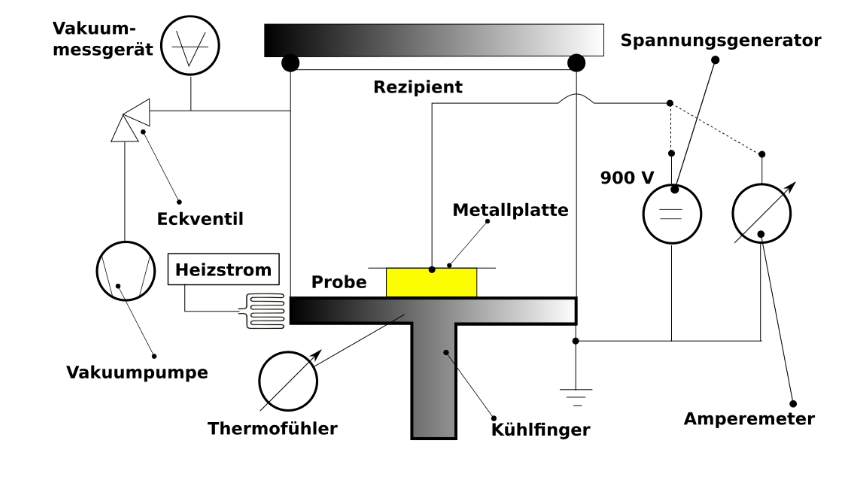
\includegraphics[scale=0.3]{content/Aufbau.png}
    \caption{Schematische Darstellung der Messvorichtung zur Dipolrelaxation \cite{Anleitung}.}
    \label{fig:Aufbau}
  \end{figure}

Im Folgenden wird die Kaliumbromidprobe betrachtet. Die Probe ist auf den Boden des Rezipienten aufgekittet. Der Rezipient ist vakuumiert, um 
Kondensation von Wasser und eine daraus resultierende Verfälschung zu verhindern. Zusammen mit einer Metallplatte, die sich auf der Probe 
befindet, bildet der Rezipient ein Plattenkondensator. Dieser ist zunächst mit einer Gleichspannungsquelle und später mit einem Pikoamperemeter 
verschaltet. Die Temperatur der Probe lässt sich mit Hilfe einer Heizspule über ein Netzgerät erhöhen. Das Abkühlen der Probe erfolgt über 
einen Kühlfinger aus Kupfer, welcher auf der einen Seite in Stickstoff gebadet werden kann. \\
Zunächst wird die Probe auf $\SI{320}{\kelvin}$ erhitzt, während ein E-Feld mit einer Spannung von $\SI{950}{\volt}$ anliegt. So sollen möglichst 
viele Dipole ausgerichtet werden. Während die Probe auf $\SI{230}{\kelvin}$ abgekühlt wird, bleibt die Dipolausrichtung unverändert. Im nächsten 
Schritt wird das E-Feld abgestellt und der Kondensator für 5 Minuten kurz geschlossen. Dies wird durchgeführt, weil es sich um sehr kleine Ströme
handelt, die von den Anschlüssen fern gehalten sollen. Danach wird die Probe möglichst gleichmäßig auf $\SI{330}{\kelvin}$ erwärmt. Dabei 
wird jede Minute die Probentemperatur mit einem Thermofühler, sowie der Depolarisationsstrom mithilfe eines Picoamperemeters gemessen. Die Heizrate
sollte dabei nicht $\SI{2}{\kelvin\per\minute}$ überschreiten.  